\documentclass[notitlepage, reprint, nofootinbib]{revtex4-1}
\usepackage[utf8]{inputenc}

% Mathematics and symbols:
\usepackage{amsmath, gensymb, amsthm, physics, mhchem}
% Figures:
\usepackage{tikz, graphicx}
\usepackage[caption=false]{subfig}

% Other:
\usepackage{hyperref}

\hypersetup{
    colorlinks=true,
    linkcolor=purple,
    filecolor=magenta,      
    urlcolor=purple,
}

\usepackage{algorithm}
\usepackage{algpseudocode}


% Document formatting 
\setlength{\parskip}{1mm}
\setlength{\parindent}{0mm}


%\renewcommand{\thesubsubsection}{\alph{subsubsection})}


\begin{document}
\title{FYS3150 - Project 4}
\author{Frida Larsen}

\begin{abstract}
This report implements the two dimensional Ising model and studies its magnetic phase transitions using Monte Carlo methods and the Metropolis algorithm. The implementation successfully reproduces the phase transition in the expected temperature region. The critical temperature of the phase transition was found to be $T_C\approx 2.271\pm0.002\ k_B/J$, which is consistent with the analytical result $T_C\approx 2.269\ k_B/J$. The results were produced using $10^6$ Monte Carlo cycles using finite grid sizes $L=$40, 60, 80 and 100. 
\end{abstract}

\maketitle

\section{Introduction}
The aim of this project is to implement and study the Ising model in two dimensions. The two dimensional Ising model exhibits a magnetic phase transition, as shown by Lars Onsager in 1944\cite{Onsager}, and is widely popular for studying this phenomenon.\\[2mm]
All relevant code may be found in the GitHub repository 'FYS3150-Computational-Physics'\footnote{\href{GitHub Repository}{https://github.com/fridalarsen/FYS3150-Computational-Physics}} under the Project4 folder. This folder also includes a Figures folder, which holds all the figures presented in this text and produced during the project. The Ising model is implemented as a class which may be found in the '\texttt{ising\_model.cpp}'-program.


\section{Theory: The Ising Model}
As previously mentioned, the Ising model is widely used for simulating phase transitions. Spins in a 2D lattice are represented by arrows pointing up or down. $\uparrow$ indicates a spin value of 1, whilst $\downarrow$ indivates a spin value of -1. \\[2mm]
In the Ising model, assuming no externally applied magnetic field, the energy of a given spin configuration $i$ can be expressed as 
\begin{equation}\label{Ising_energy}E_i=-J\sum_{<kl>}^Ls_ks_l,\end{equation}
where $L$ is the total number of spins in the system, $J$ is a coupling constant. $s_k$ and $s_l$ are the values of the spins, and can be $\pm1$. The sum is over neighbouring spins, and each pair $k,l$ are counted only once. \\[2mm]
For this project, we will use periodic boundary conditions\footnote{Another option is free ends. The way the boundaries are treated become less significant for larger systems.}. See figure \ref{sketch} for an illustration of the 2x2 case.\\[2mm]
The magnetization of a given configuration is given by
\begin{equation}\label{magnetization}\mathcal{M}_i=\sum_{k=1}^N s_k.\end{equation}

\begin{figure} 
	\centering
	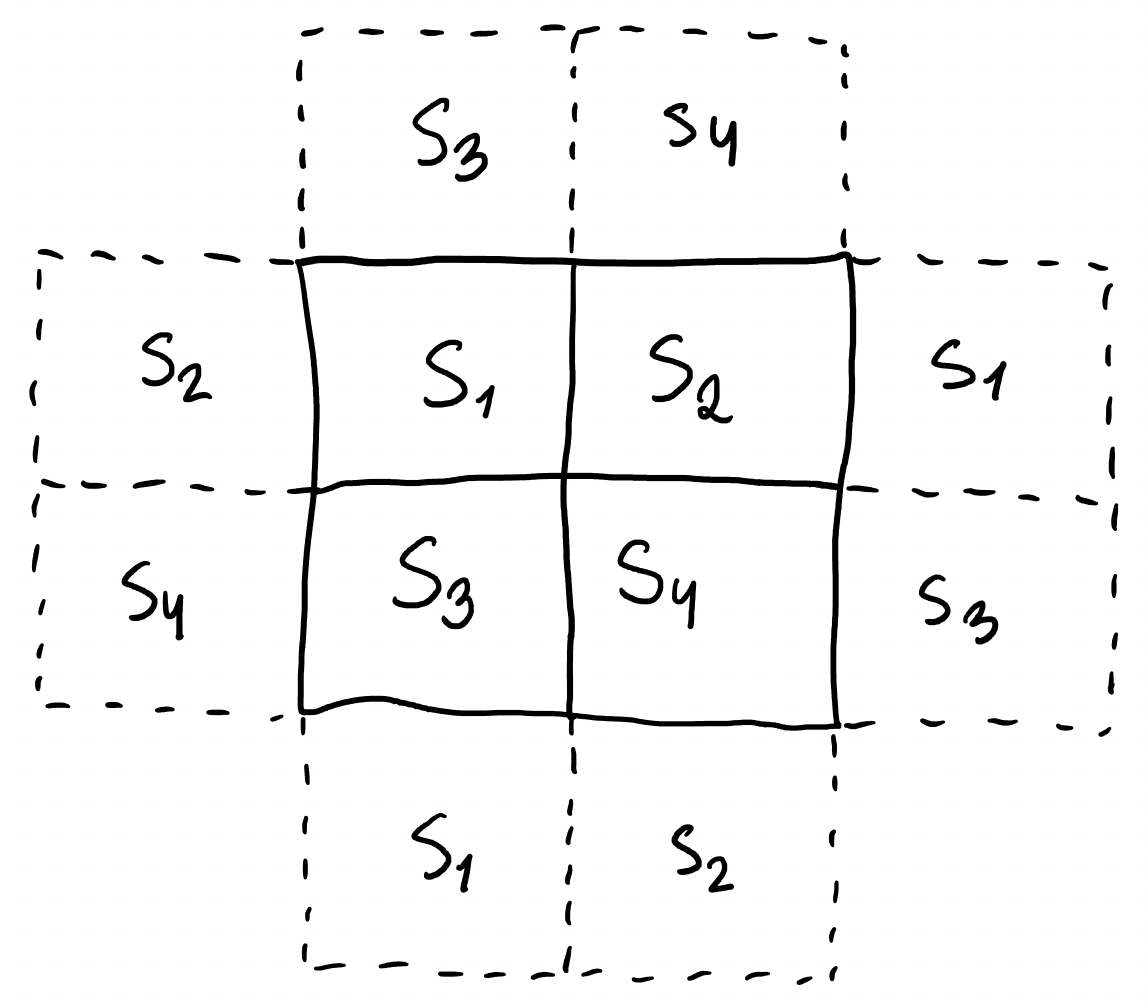
\includegraphics[width=0.35\textwidth]{../Figures/pbc_sketch.png}
	\caption{Illustration of periodic boundary conditions on a $2\times2$ grid.}
	\label{sketch}
\end{figure}

\subsection{Statistical Physics}
The statiscial properties of a system in thermal equilibrium are described by the partition function, 
\begin{equation}\label{partition_function}Z=\sum_{i=1}^M e^{-\beta E_i},\end{equation}
where $M$ is the total number of microstates. $\beta$ is a constant, given by 
\begin{equation}\label{beta}\beta=\frac{1}{k_BT}.\end{equation}
The partition function can be used to deduct a number of other interesting properties of the system. The mean energy and the mean squared energy are given by 
\begin{equation}\label{mean_energy}\langle E\rangle =\frac{1}{Z}\sum_{i=1}^ME_ie^{-\beta E_i}\end{equation}
and
\begin{equation}\label{mean_energy_2}\langle E^2\rangle = \frac{1}{Z}\sum_{i=1}^M E_i^2 e^{-\beta E_i}.\end{equation}
The mean magnetization is 
\begin{equation}\label{mean_mag}\langle \mathcal{M}\rangle =\frac{1}{Z}\sum_{i=1}^M\mathcal{M}_i e^{\beta E_i},\end{equation}
where $\mathcal{M}_i$ is given by equation \ref{magnetization}. The mean of the magnetization squared is given by 
\begin{equation}\label{mean_mag2}\langle \mathcal{M}^2\rangle =\frac{1}{Z}\sum_{i=1}^M\mathcal{M}_i^2 e^{\beta E_i},\end{equation}
This project is particularly interested in two properties, namely the specific heat and the magnetic susceptibility.\\[2mm]
The specific heat, $C$, of a system is the amount of energy that must be added to the system in order to increase the temperature of one matter unit by one temperature unit. If the substance being heated is allowed to expand as it is being heated, the specific heat is said to be at constant pressure. If the substance is heated in an enclosed space, however, the specific hest is said to be at constant volume. In the latter case, the specific heat is given by 
\begin{equation}\label{specific_heat}C_V = \frac{1}{k_BT^2}(\langle E^2\rangle - \langle E\rangle^2).\end{equation}
The susceptibility of a substance is a measure of how much the material will become magnetized if a magnetic field is applied and is given by 
\begin{equation}\label{susceptibility}\chi = \beta (\langle \mathcal{M}^2\rangle -\langle \mathcal{M}\rangle^2).\end{equation}

\subsection{The 2x2 case}
Consider a 2x2 lattice of spins. There are $2^4=16$ possible configurations. The expression for the energy from equation \ref{Ising_energy} can be written out as 
\begin{align}
	E_i = &s_1s_2+s_2s_1+s_3s_4+s_4s_3\nonumber \\
	&+s_3s_1+s_1s_3+s_2s_4+s_4s_2\label{Ising_energy_2x2}
\end{align}
where the spins are labeled as in figure \ref{sketch}. Table \ref{2x2_table} lists the degeneracy, energy and magnetization of each possible configuration. 
\begin{table}[]
\centering
\begin{tabular}{|l|l|l|l|}
\hline
Number of $\uparrow$ & Degeneracy & Energy ($E_i$) & Magnetization ($\mathcal{M}_i$) \\ \hline
4 & 1 & -8J & 4 \\ \hline
3 & 4 & 0 & 2 \\ \hline
2 & 4 & 0 & 0 \\ \hline
2 & 2 & 8J & 0 \\ \hline
1 & 4 & 0 & -2 \\ \hline
0 & 1 & -8J & -4 \\ \hline
\end{tabular}
\caption{Degeneracy, energy and magnetization of all configurations of spins in a 2x2 lattice.}
\label{2x2_table}
\end{table}
The partition function is given by 
\begin{align*}
	Z_{2x2}&=e^{-\beta(-8J)}+4e^0+4e^0+2e^{-\beta(8J)}+4e^0+e^{-\beta(-8J)}\\
	&= 2e^{8\beta J}+2e^{-8\beta J}+12.
\end{align*}
The mean energy and the mean squared energy is given by 
\begin{align*}
	\langle E\rangle&=\frac{-8Je^{8\beta J}+16Je^{-8\beta J}-8Je^{8\beta J}}{2e^{8\beta J}+2e^{-8\beta J}+12}\\
	&=\frac{8Je^{-8\beta J} - 8Je^{8\beta J}}{e^{8\beta J}+e^{-8\beta J}+6}
\end{align*}
and 
\begin{align*}
	\langle E^2\rangle &=\frac{(-8J)^2e^{8\beta J}+2(8J)^2e^{-8\beta J}+(-8J)^2e^{8\beta J}}{2e^{8\beta J}+2e^{-8\beta J}+12}\\
	&=\frac{64J^2e^{-8\beta J} + 64J^2e^{8\beta J}}{e^{8\beta J}+e^{-8\beta J}+6}.
\end{align*}
Thus the specific heat capacity becomes 
\begin{equation*} C_V=\frac{1}{k_BT^2}\Big(\frac{64J^2e^{-8\beta J} + 64J^2e^{8\beta J}}{e^{8\beta J}+e^{-8\beta J}+6} - \Big[\frac{8Je^{-8\beta J} - 8Je^{8\beta J}}{e^{8\beta J}+e^{-8\beta J}+6}\Big]^2\Big).\end{equation*}
For the mean magnetization and the mean square magnetization we get 
\begin{align*}
	\langle M\rangle &= \frac{4e^{8\beta J}+2e^0-2e^0-4e^{8\beta J}}{2e^{8\beta J}+2e^{-8\beta J}+12}\\
	&=0
\end{align*}
and
\begin{align*}
	\langle M^2 \rangle &=\frac{16e^{-8\beta J}+4e^0+4e^0+16e^{8\beta J}}{2e^{8\beta J}+2e^{-8\beta J}+12}\\
	&= \frac{8e^{-8\beta J}+8e^{8\beta J}+4}{e^{8\beta J}+e^{-8\beta J}+6}.
\end{align*}
Thus the susceptibility becomes 
\begin{align*}
	\chi &= \frac{1}{k_BT}\Big(\frac{8e^{-8\beta J}+8e^{8\beta J}+4}{e^{8\beta J}+e^{-8\beta J}+6} - 0\Big)\\
	&=\frac{1}{k_BT} \frac{8e^{-8\beta J}+8e^{8\beta J}+4}{e^{8\beta J}+e^{-8\beta J}+6}.
\end{align*}

\subsection{Phase transitions}
The 2D Ising model has a phase transition of second order. At a given temperature the system will transition from a magnetic phase with finite magnetic moment to a phase with zero magnetization. The temperature above which the mean magnetization is zero is called the critical temperature, $T_C$. \\[2mm]
Near $T_C$, the statistical properties $\mathcal{M}$, $C_V$ and $\chi$ all behave according to power laws. For infinite grid sizes we have\cite{lecture_notes}
\begin{equation}\label{m1}\langle M(T)\rangle \sim (T-T_C)^\beta,\end{equation}
\begin{equation}\label{c1}C_V(T)\sim |T_C-T|^\alpha,\end{equation}
and
\begin{equation}\label{chi1}\chi(T)\sim |T_C-T|^\gamma,\end{equation}
where $\beta=1/8$, $\alpha=0$ and $\gamma=7/4$. The critical temperature for finite grids will deviate slightly from that of an infinite grid. The difference scales as 
\begin{equation}\label{T_C}T_C(L)-T_C(L=\infty)=aL^{-1/\nu},\end{equation}
where $a$ is some constant and $\nu=1$. Inserting this into equations \ref{m1}, \ref{c1} and \ref{chi1} we get 
\begin{equation}\label{m2}\langle \mathcal{M}(T)\rangle \sim L^{-\beta/\nu},\end{equation}
\begin{equation}\label{c2}[C_V(T)]^{-1}\sim L^{\alpha/\nu}\end{equation}
and
\begin{equation}\label{chi2}[\chi(T)]^{-1}\sim L^{\gamma/\nu}.\end{equation}
The exact result for the critical temperature is\cite{Onsager} 
\begin{equation}\label{onsager_tc}\frac{kT_C}{J}=\frac{2}{\ln (1+\sqrt{2})}\approx2.269\end{equation}

\section{Method}
The goal is to calculate the expectation values $\langle E\rangle$, $\langle E^2\rangle$, $\langle |\mathcal{M}|\rangle$ and $\langle\mathcal{M}^2\rangle$ numerically using Monte Carlo methods. The general expression for the expected value of some function $f(x)$, where $x$ is distributed according to some probability density $p(x)$, is given by
\begin{equation}\label{exp_val}\langle f(x)\rangle =\sum_i f(x_i)p(x_i),\end{equation}
The Monte Carlo estimate for this expectation value is 
\begin{equation}\label{MC}\langle f(x)\rangle \approx \frac{1}{N}\sum_j f(x_j).\end{equation}
where $x_j$ is drawn from the same probability density $p(x)$. In our case, $x_j$ is a configuration of $L\times L$ spins in a lattice. In order to find the most probable configurations for a particular temperature, we use the Metropolis algorithm as follows;
\begin{algorithm}[H]
	\caption{Metropolis algorithm for spin flipping}
	\begin{algorithmic}[1]
		\State Choose a random spin in the lattice and flip it.
		\State Compute the energy change, $\Delta E$, caused by the flip.
		\If{$\Delta E\leq0$}
			\State The flip is accepted, update expectation values. 
		\ElsIf{$\Delta E\geq 0$}
			\State Calculate $w=e^{-\beta\Delta E}$.
			\State Draw a random number $r$.
			\If{$r\leq w$}
				\State The flip is accepted, update expectation values.
			\Else
				\State Revert back to previous configuration.
			\EndIf
		\EndIf
	\end{algorithmic}
\end{algorithm}
The variable $\beta$ is given by equation \ref{beta}.\\[2mm]
Before each Monte Carlo cycle it is neccessary to randomize the grid by performing a set number, $n$, of spin flips in order to make sure that the random properties of the Metropolis algorithm are kept intact. We have chosen to use $n=L\times L$ as this scales nicely with the grid size. 

\section{Results}
The numerical calculation of the mean energy, mean absolute magnetization, specific heat and susceptibility are compared to the analytic values in figures \ref{fig1}, \ref{fig2}, \ref{fig3} and \ref{fig4}. We see a significant leap in accuracy around $10^4$ for all four thermodynamic variables. \\[2mm]
The evolution of the total energy and magnetization of a randomized $20\times20$ lattice for $T=1.0$ is shown in figures \ref{fig5} and \ref{fig6}. The plots for $T=1.0$ starting with an organized grid, as well as the plots for $T=2.4$ may be found in the Figures folder\footnote{The relevant plots are labeled 4c.}, as mentioned in the introduction. However, they do not show a clear transition to equilibrium like the $T=1.0$ with randomized grid plots do. We see from these two plots that equilibrium is reached after roughly 1000 Monte Carlo cycles. \\[2mm]
Figure \ref{fig7} shows the number of spin flips accepted by the Metropolis algorithm as a function of number of Monte Carlo cycles for two different temperatures, for both organized and randomized initital configurations. We see that the lower temperature has a lower acceptance rate for both the initial configurations.\\[2mm]
The probability for a given energy to appear in the computations after equilibrium has been reached are presented in figures \ref{fig8} and \ref{fig9} for $T=1.0$ and $T=2.4$ respectively. The variance is indicated as labels. We see that the distribution for $T=1.0$ seems to be exponential, whilst the distribution for $T=2.4$ seems to be Gaussian.\\[2mm]
Figure \ref{fig10} shows the specific heat during a phase transition for $L=100$. The phase transition plots for the susceptibility, mean energy and mean absolute magnetization for $L=40,\ 60,\ 80$ and 100 may be found in the Figures folder\footnote{The relevant plots are labeled 4e.}. The same applies to the specific heat plots for the former three.\\[2mm]
The estimated $T_C$-values from the plots of $C_V$ and $\chi$ can be found in table \ref{T_C_table}. The average values from the table is plotted as a function of 1/L in figure \ref{fig11} along with the regression line\cite{Squires}. By equation \ref{T_C} we find 
$$T_C\approx 2.271\pm0.002\ k_B/J$$
We observe that the analytical result (equation \ref{onsager_tc}) is within the confidence interval of this result.

\begin{figure} %4b
	\centering
	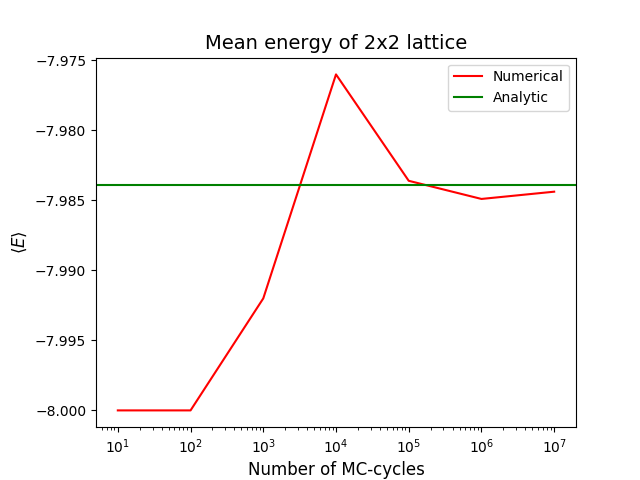
\includegraphics[width=0.45\textwidth]{../Figures/E_mean_4b.png}
	\caption{The mean energy of a 2x2 lattice computed numerically and analytically}
	\label{fig1}
\end{figure}

\begin{figure} %4b
	\centering
	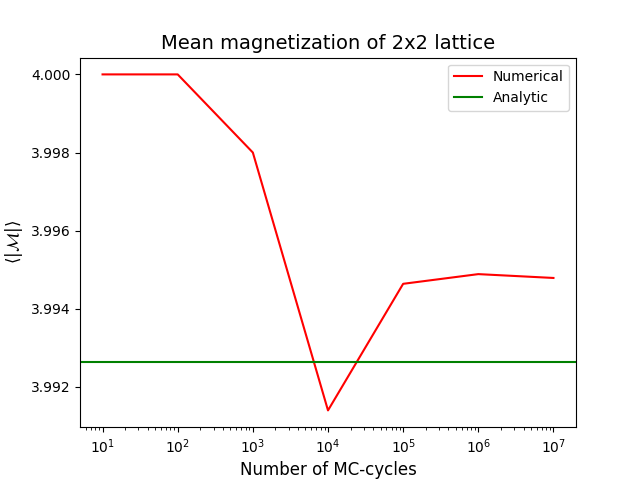
\includegraphics[width=0.45\textwidth]{../Figures/M_mean_4b.png}
	\caption{The mean absolute magnetization of a 2x2 lattice computed numerically and analytically}
	\label{fig2}
\end{figure}

\begin{figure} %4b
	\centering
	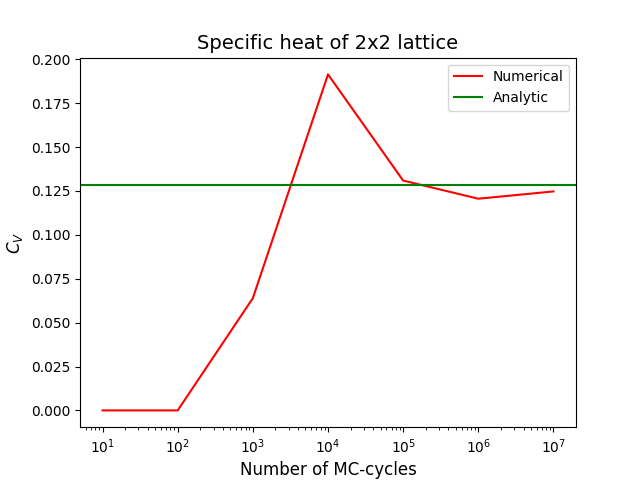
\includegraphics[width=0.45\textwidth]{../Figures/C_V_4b.png}
	\caption{The specific heat of a 2x2 lattice computed numerically and analytically}
	\label{fig3}
\end{figure}

\begin{figure} %4b
	\centering
	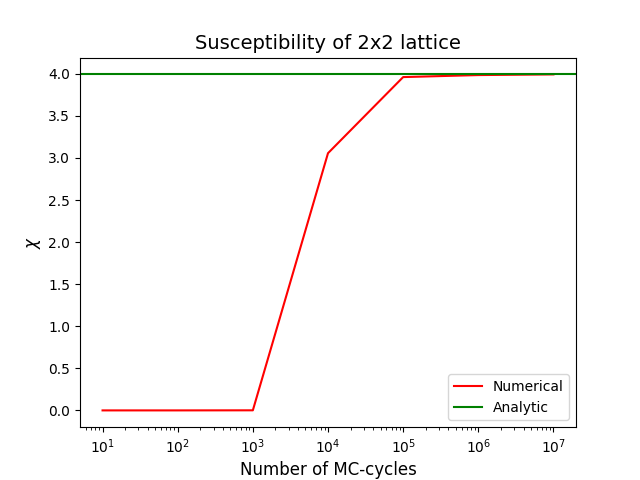
\includegraphics[width=0.45\textwidth]{../Figures/chi_4b.png}
	\caption{The susceptibility of a 2x2 lattice computed numerically and analytically}
	\label{fig4}
\end{figure}

\begin{figure}%4c
	\centering 
	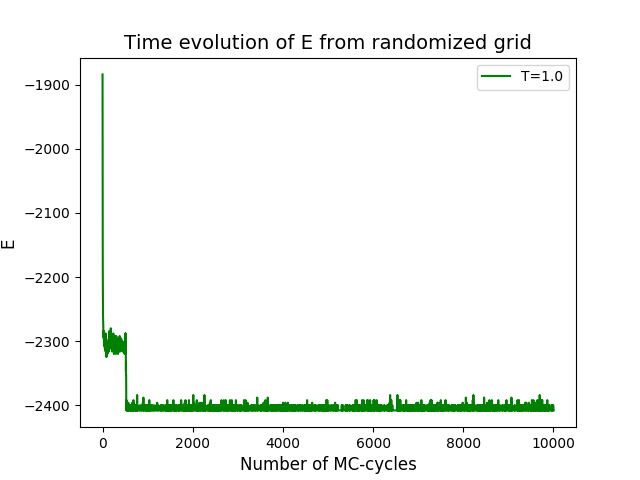
\includegraphics[width=0.45\textwidth]{../Figures/4c_E2.png}
	\caption{Evolution of total energy of lattice for T=1.0 from a randomized grid.}
	\label{fig5}
\end{figure}

\begin{figure}%4c
	\centering 
	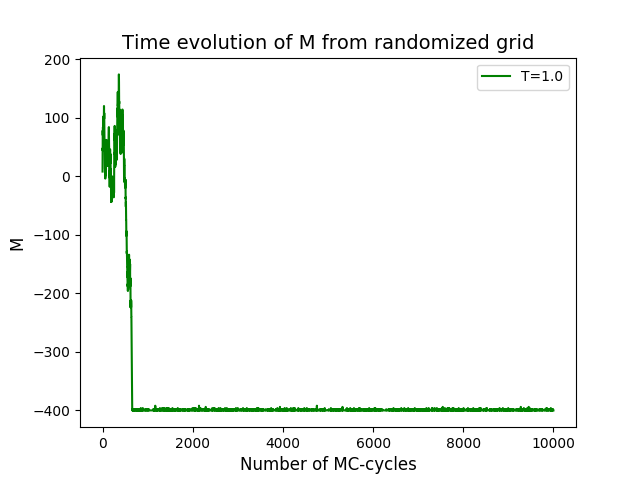
\includegraphics[width=0.45\textwidth]{../Figures/4c_M2.png}
	\caption{Evolution of total magnetization of lattice for T=1.0 from a randomized grid.}
	\label{fig6}
\end{figure}

\begin{figure}%4c
	\centering 
	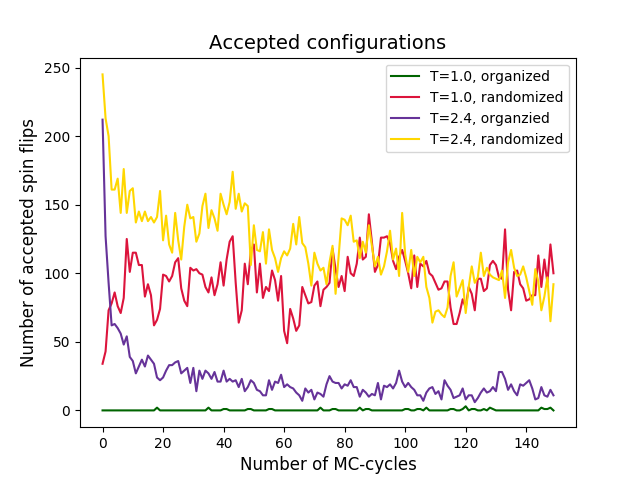
\includegraphics[width=0.45\textwidth]{../Figures/4c_accepted_config.png}
	\caption{Accepted spin configurations from the Metropolis algorithm.}
	\label{fig7}
\end{figure}

\begin{figure}%4d
	\centering 
	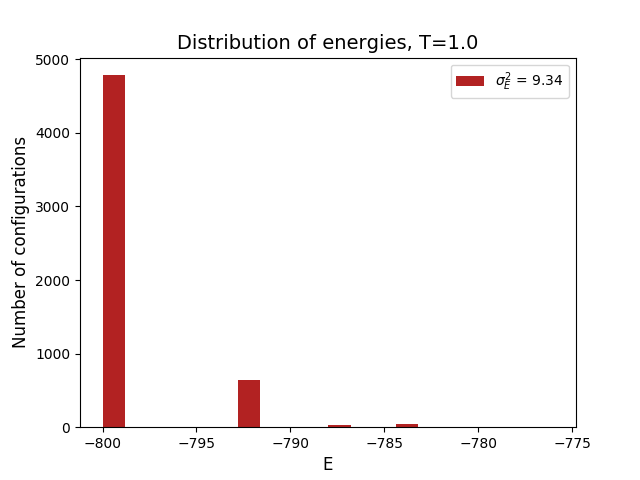
\includegraphics[width=0.45\textwidth]{../Figures/4d_histogram_T1.png}
	\caption{Frequency of certain energies for a $20\times20$ lattice at $T=1.0$.}
	\label{fig8}
\end{figure}

\begin{figure}%4d
	\centering 
	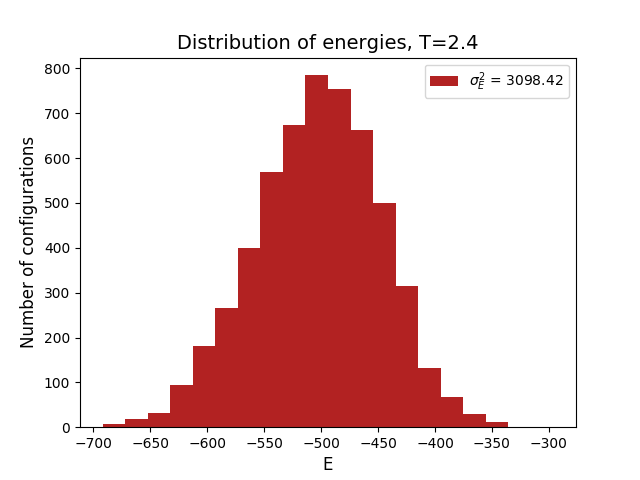
\includegraphics[width=0.45\textwidth]{../Figures/4d_histogram_T2.png}
	\caption{Frequency of certain energies for a $20\times20$ lattice at $T=2.4$.}
	\label{fig9}
\end{figure}

\begin{figure}%4e
	\centering 
	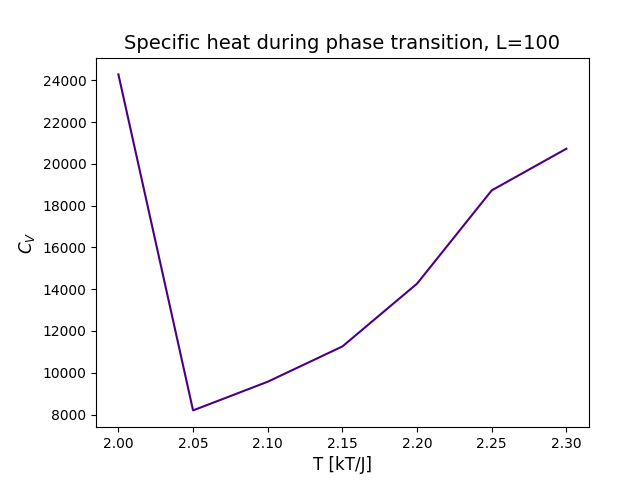
\includegraphics[width=0.45\textwidth]{../Figures/4e_L100_2.png}
	\caption{The specific heat of a lattice during phase transition with $L=100$.}
	\label{fig10}
\end{figure}

\begin{table}[] %4f
\centering
\begin{tabular}{|l|l|l|l|}
\hline
$L$ & $T_C$ from $C_V$ & $T_C$ from $\chi$ & Average $T_C$ \\ \hline
40 & 2.28551724 & 2.24206897 & 2.2637931 \\ \hline
60 & 2.28344828 & 2.25034483 & 2.26689655 \\ \hline
80 & 2.28137931 & 2.25655172 & 2.26896552 \\ \hline
100 & 2.27103448 & 2.26275862 & 2.26689655 \\ \hline
\end{tabular}
\caption{Estimates of critical temperatures in units of $k_B/J$ of finite grids.}
\label{T_C_table}
\end{table}

\begin{figure}%4f
	\centering 
	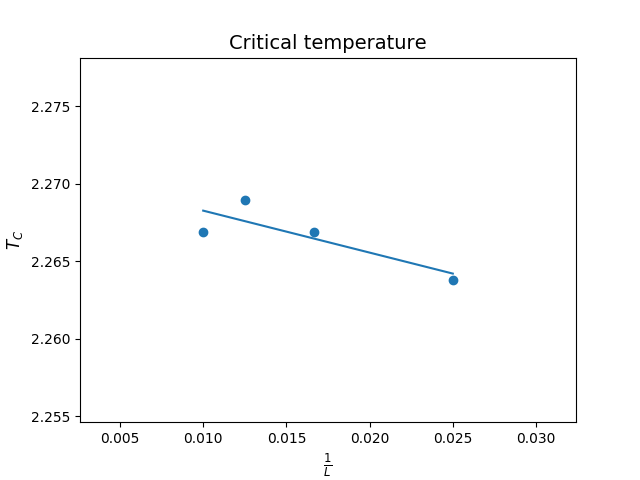
\includegraphics[width=0.45\textwidth]{../Figures/critical_temp.png}
	\caption{Estimate of critical temperature}
	\label{fig11}
\end{figure}

\clearpage
\section{Discussion}
The plots showing the analytical vs the numerical results for a $2\times2$ lattice shows us that the numerical model tends to the analytical result as the number of Monte Carlo cycles crosses $10^5$. This shows that our model successfully replicates the analytical system. From figures \ref{fig5} and \ref{fig6} we saw that a Monte Carlo burn in of approximately 1000 cycles was sufficient to bring the system to an equilibrium state. \\[2mm]
We found that a higher temperature gave a higher acceptance rate from the Metropolis algorithm. The temperatures were above and below the analytical critical temperature for the magnetic phase transition. This is reflected in our finding that while the grid for the lower temperature tends to remain stable, the grid for the higher temperature tends to fluctuate between states about the equilibirum. As with the tendency towards the analytical results previously mentioned, this is another indication that our model is successfully implemented. Further evidence of this is found in the energy distributions (figures \ref{fig8} and \ref{fig9}), which mach theoretical predictions. From these plots and the variances we see again the energy fluctuation of the higher temperature.\\[2mm] 
The critical temperatures found from the specific heat and susceptibility were constantly over and under the analytical critical temperature for all $L$-values tested. \\[2mm]
Some of the phase transition plots had noticeable jumps and dips, which is probably a result of too few Monte Carlo cycles. However, the long run time made it unfeasible to run more than $10^6$ cycles, even though our results were calculated using two parallel processes. An improved algorithm or a computer able to run more than two processes in parallel may improve the numerical stability of the data. \\[2mm]
In our simulation the average $T_C$-value calculated from the $C_V$ and $\chi$ plots happened to fall close to the analytical value of $T_C$ (equation \ref{onsager_tc}). This stems from how the $T_C$-value calculated from the $C_V$ and $\chi$ plots were symmetrically skewed above and below the analytical $T_C$-value by the same amount. However, it is unclear whether this is a result of using a finite grid or by random chance. 

\section{Conclusion}
The aim of this project was to implement and study the Ising model for a 2D grid in order to study its phase transitions. Our implementation reproduced analytical results for the $2\times2$-system to a sufficient accuracy. The numerical simulations showed clear signs of the theoretical magnetic phase transition, such as fluctuating equilibrium states for higher temperatures and critical behaviour of $C_V$ and $\chi$ for temperatures close to $T_C$. Although the critical temperature was reproduced to a significant accuracy, the validity of this result is questionable due to the error-prone algorithm with which it was determined. \\[2mm]
Future projects should aim to improve the accuracy of the phase transition data, using more Monte Carlo cycles and studying smaller temperature intervals. Improvements can also be made to the determination of $T_C$ from the $C_V$ and $\chi$ plots, for instance using regression instead of simply selecting the largest data point.

\onecolumngrid
\bibliographystyle{unsrtnat}
\bibliography{references.bib}









\end{document}